\documentclass{sigchi}

% Use this command to override the default ACM copyright statement (e.g. for preprints). 
% Consult the conference website for the camera-ready copyright statement.


%% EXAMPLE BEGIN -- HOW TO OVERRIDE THE DEFAULT COPYRIGHT STRIP -- (July 22, 2013 - Paul Baumann)
% \toappear{Permission to make digital or hard copies of all or part of this work for personal or classroom use is 	granted without fee provided that copies are not made or distributed for profit or commercial advantage and that copies bear this notice and the full citation on the first page. Copyrights for components of this work owned by others than ACM must be honored. Abstracting with credit is permitted. To copy otherwise, or republish, to post on servers or to redistribute to lists, requires prior specific permission and/or a fee. Request permissions from permissions@acm.org. \\
% {\emph{CHI'14}}, April 26--May 1, 2014, Toronto, Canada. \\
% Copyright \copyright~2014 ACM ISBN/14/04...\$15.00. \\
% DOI string from ACM form confirmation}
%% EXAMPLE END -- HOW TO OVERRIDE THE DEFAULT COPYRIGHT STRIP -- (July 22, 2013 - Paul Baumann)


% Arabic page numbers for submission. 
% Remove this line to eliminate page numbers for the camera ready copy
% \pagenumbering{arabic}


% Load basic packages
\usepackage{balance}  % to better equalize the last page
\usepackage{graphics} % for EPS, load graphicx instead
\usepackage{times}    % comment if you want LaTeX's default font
\usepackage{url}      % llt: nicely formatted URLs

% llt: Define a global style for URLs, rather that the default one
\makeatletter
\def\url@leostyle{%
  \@ifundefined{selectfont}{\def\UrlFont{\sf}}{\def\UrlFont{\small\bf\ttfamily}}}
\makeatother
\urlstyle{leo}


% To make various LaTeX processors do the right thing with page size.
\def\pprw{8.5in}
\def\pprh{11in}
\special{papersize=\pprw,\pprh}
\setlength{\paperwidth}{\pprw}
\setlength{\paperheight}{\pprh}
\setlength{\pdfpagewidth}{\pprw}
\setlength{\pdfpageheight}{\pprh}

% Make sure hyperref comes last of your loaded packages, 
% to give it a fighting chance of not being over-written, 
% since its job is to redefine many LaTeX commands.
\usepackage[pdftex]{hyperref}
\hypersetup{
pdftitle={SIGCHI Conference Proceedings Format},
pdfauthor={LaTeX},
pdfkeywords={SIGCHI, proceedings, archival format},
bookmarksnumbered,
pdfstartview={FitH},
colorlinks,
citecolor=black,
filecolor=black,
linkcolor=black,
urlcolor=black,
breaklinks=true,
}

% create a shortcut to typeset table headings
\newcommand\tabhead[1]{\small\textbf{#1}}


% End of preamble. Here it comes the document.
\begin{document}

\title{FeedLearn: Microlearning while Browsing Social Feeds}

\numberofauthors{3}
\author{
  \alignauthor 1st Author Name\\
    \affaddr{Affiliation}\\
    \affaddr{Address}\\
    \email{e-mail address}\\
    \affaddr{Optional phone number}
  \alignauthor 2nd Author Name\\
    \affaddr{Affiliation}\\
    \affaddr{Address}\\
    \email{e-mail address}\\
    \affaddr{Optional phone number}    
  \alignauthor 3rd Author Name\\
    \affaddr{Affiliation}\\
    \affaddr{Address}\\
    \email{e-mail address}\\
    \affaddr{Optional phone number}
}

\maketitle

\begin{abstract}
Many long-term goals, such as learning a new language,
require the person to spend a small amount of time each day to achieve them.
At the same time, people regularly browse social news feeds in their spare time, or otherwise
engage in online media consumption that is unrelated to the user's work.
Our system, FeedLearn, exploits the regularity with which people spend their idle time reading news feeds on Facebook,
in order to present them with microlearning tasks. We find that over the course of 2 weeks, we are able to teach students N new vocabulary words by injecting microlearning tasks into their Facebook feeds. This is X\% more than a control condition where we ask them to visit a separate website and ask them to study the words on their own time, and Y\% more than a control condition where we also remind them to visit the website to review via feed updates.

\end{abstract}

\keywords{
	microlearning; social feeds; language learning
}

\category{H.5.m.}{Information Interfaces and Presentation (e.g. HCI)}{Miscellaneous}

%See: \url{http://www.acm.org/about/class/1998/}
%for more information and the full list of ACM classifiers
%and descriptors. \newline
%\textcolor{red}{Optional section to be included in your final version, 
%but strongly encouraged. On the submission page only the classifiers’ 
%letter-number combination will need to be entered.}

\section{Introduction}

People spend large amounts of time online on activities not related to work,
which is commonly referred to as ``cyberslacking''.
Studies have found that the majority of internet time at work is spent cyberslacking,
and that usage of social networking sites
constitutes a large portion of cyberslacking activity, particularly among younger employees \cite{cyberslacking}. Over 90\% of college students use Facebook \cite{collegefacebook2}. College students who use Facebook report spending an average of 30 minutes per day on Facebook, and the majority check their news feeds 5-7 days each week \cite{collegefacebook}. Clearly, Facebook news feeds present an opportunity for influencing the behavior of users.

In this paper, we present FeedLearn, a mechanism for allowing users to study flashcard-like content, such as vocabulary, as they browse through their Facebook feeds. We compared foreign-vocabulary acquisition rates through FeedLearn to simply asking users to study them on an external web service, and found that users learned X\% more vocabulary with FeedLearn.

\section{Related Work}

\subsection{News Feeds as a Persuasive Technology}

Since the emergence of the Facebook app development platform, there have been
many attempts to use it as a platform for persuasion. For example, apps like NikePlus broadcast users' running progress, and apps like Duolingo broadcast users' study progress on the platform. These messages may also invite the user's friends to participate in the activity. A key advantage that social platforms like Facebook provide over generic messaging is that friends can be associated with requests, increasing their potential persuasiveness via social pressures \cite{foggfacebook}.

However, there are many caveats with applications auto-posting messages on users' behalves. Messages auto-posted by applications receive little attention from the user's friends, compared to messages that they have posted themselves. The user's audiences may also perceive their application-associated posts as either trivial achievements or bragging, ignoring them. It is thus suggested that these auto-posted messages be shared only with the subset of the user's social circles who are actually likely to engage with them \cite{socialsharing}. However, users are often reluctant to take the effort to identify these social circles.

\subsection{Incorporating Learning Into Daily Routines}

Microlearning is a strategy of using short periods of time throughout one's everyday daily routine to study. It has been used for in-context acquisition of foreign vocabulary from the environment \cite{microlearning} \cite{micromandarin}. Wait-Learning is a related strategy where idle seconds spent waiting, such as waiting for someone to respond to a chat message, are used to learn foreign-language vocabulary \cite{waitlearning}. ALOE is a system that allows users to learn foreign-language vocabulary while browsing the web, by replacing words in the user's native language with foreign-language vocabulary \cite{augmenting}.

\section{FeedLearn Interface}

\begin{figure*}
\centering
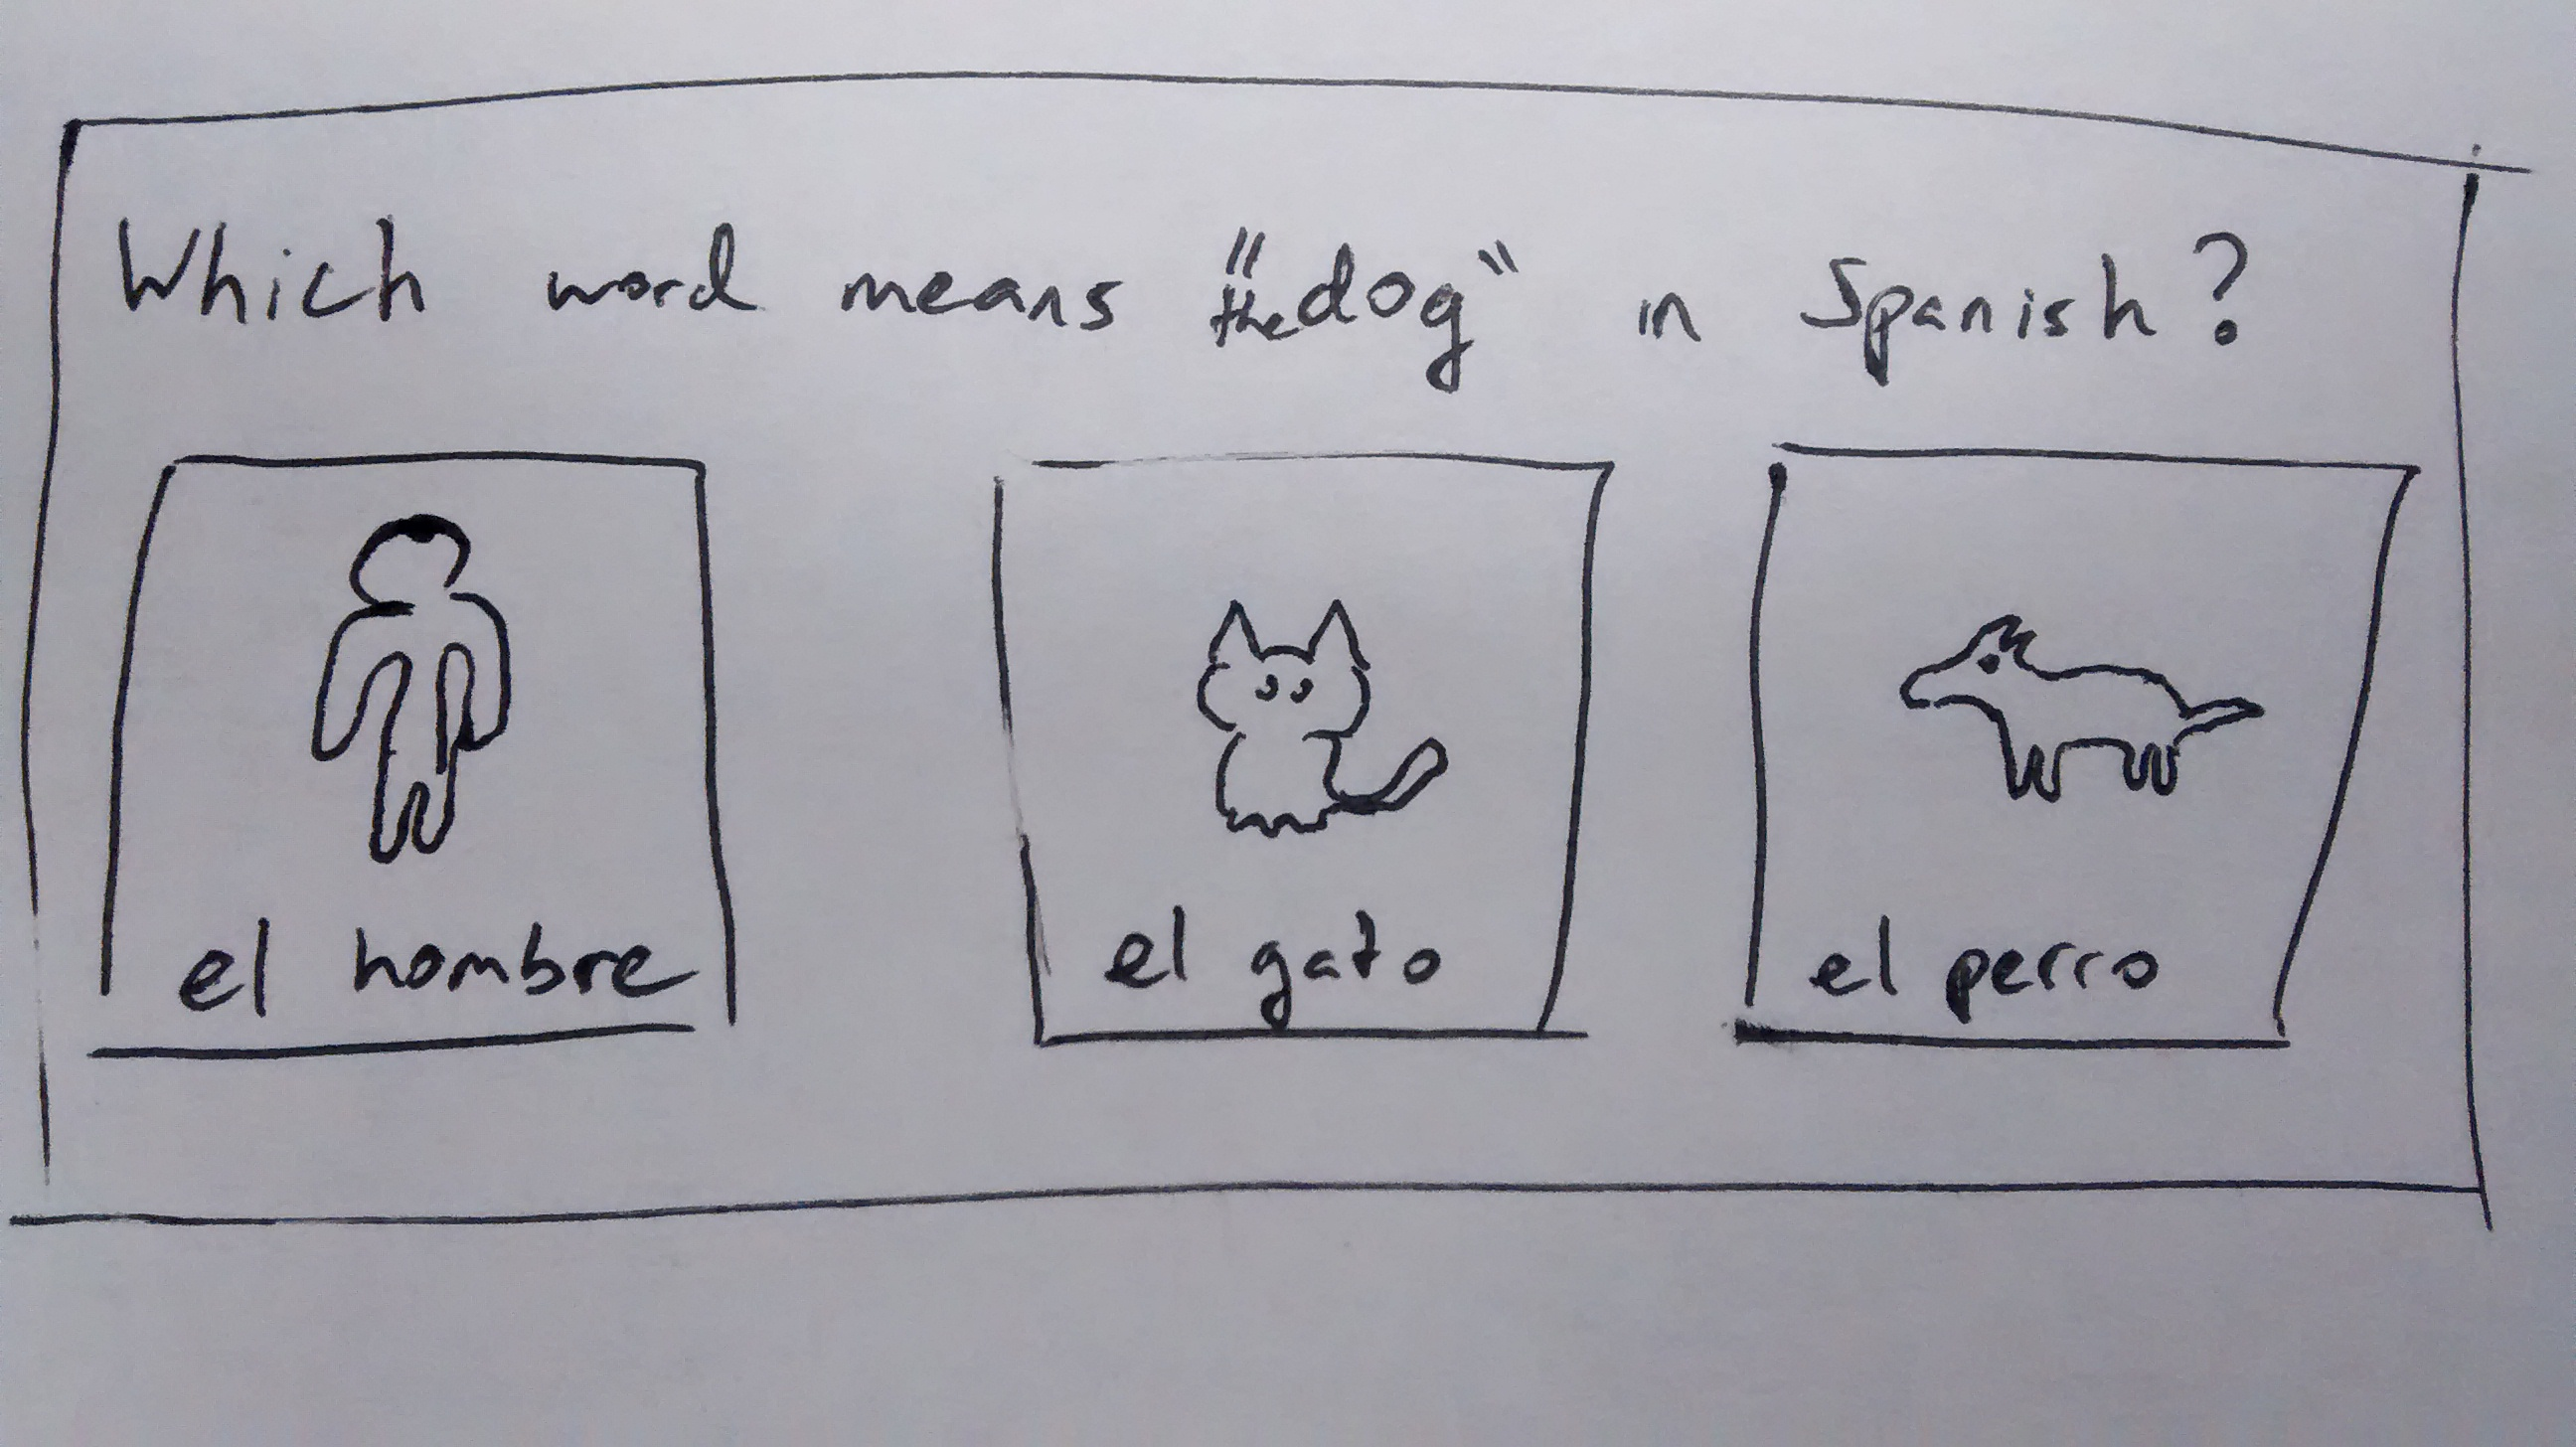
\includegraphics[width=2.0\columnwidth]{quiz1}
\caption{One type of quiz presents a noun in the native language (the dog), and asks the user to select the correct translation into the foreign language (el perro).}
\label{fig:quiz1}
\end{figure*}

FeedLearn is a Chrome extension which inserts small vocabulary quizzes into the user's Facebook feeds.

\subsection{Quiz Types}

These quizzes initially present a noun in the native language, and ask the user to select the corresponding foreign-language word, as shown in Figure~\ref{fig:quiz1}. In order to ensure that users learn to recognize the word associations in both ways, we also have a second type of quiz, in which the user is shown a word in the foreign language and selects the corresponding word in their native language, as shown in Figure~\ref{fig:quiz2}.

\begin{figure*}
\centering
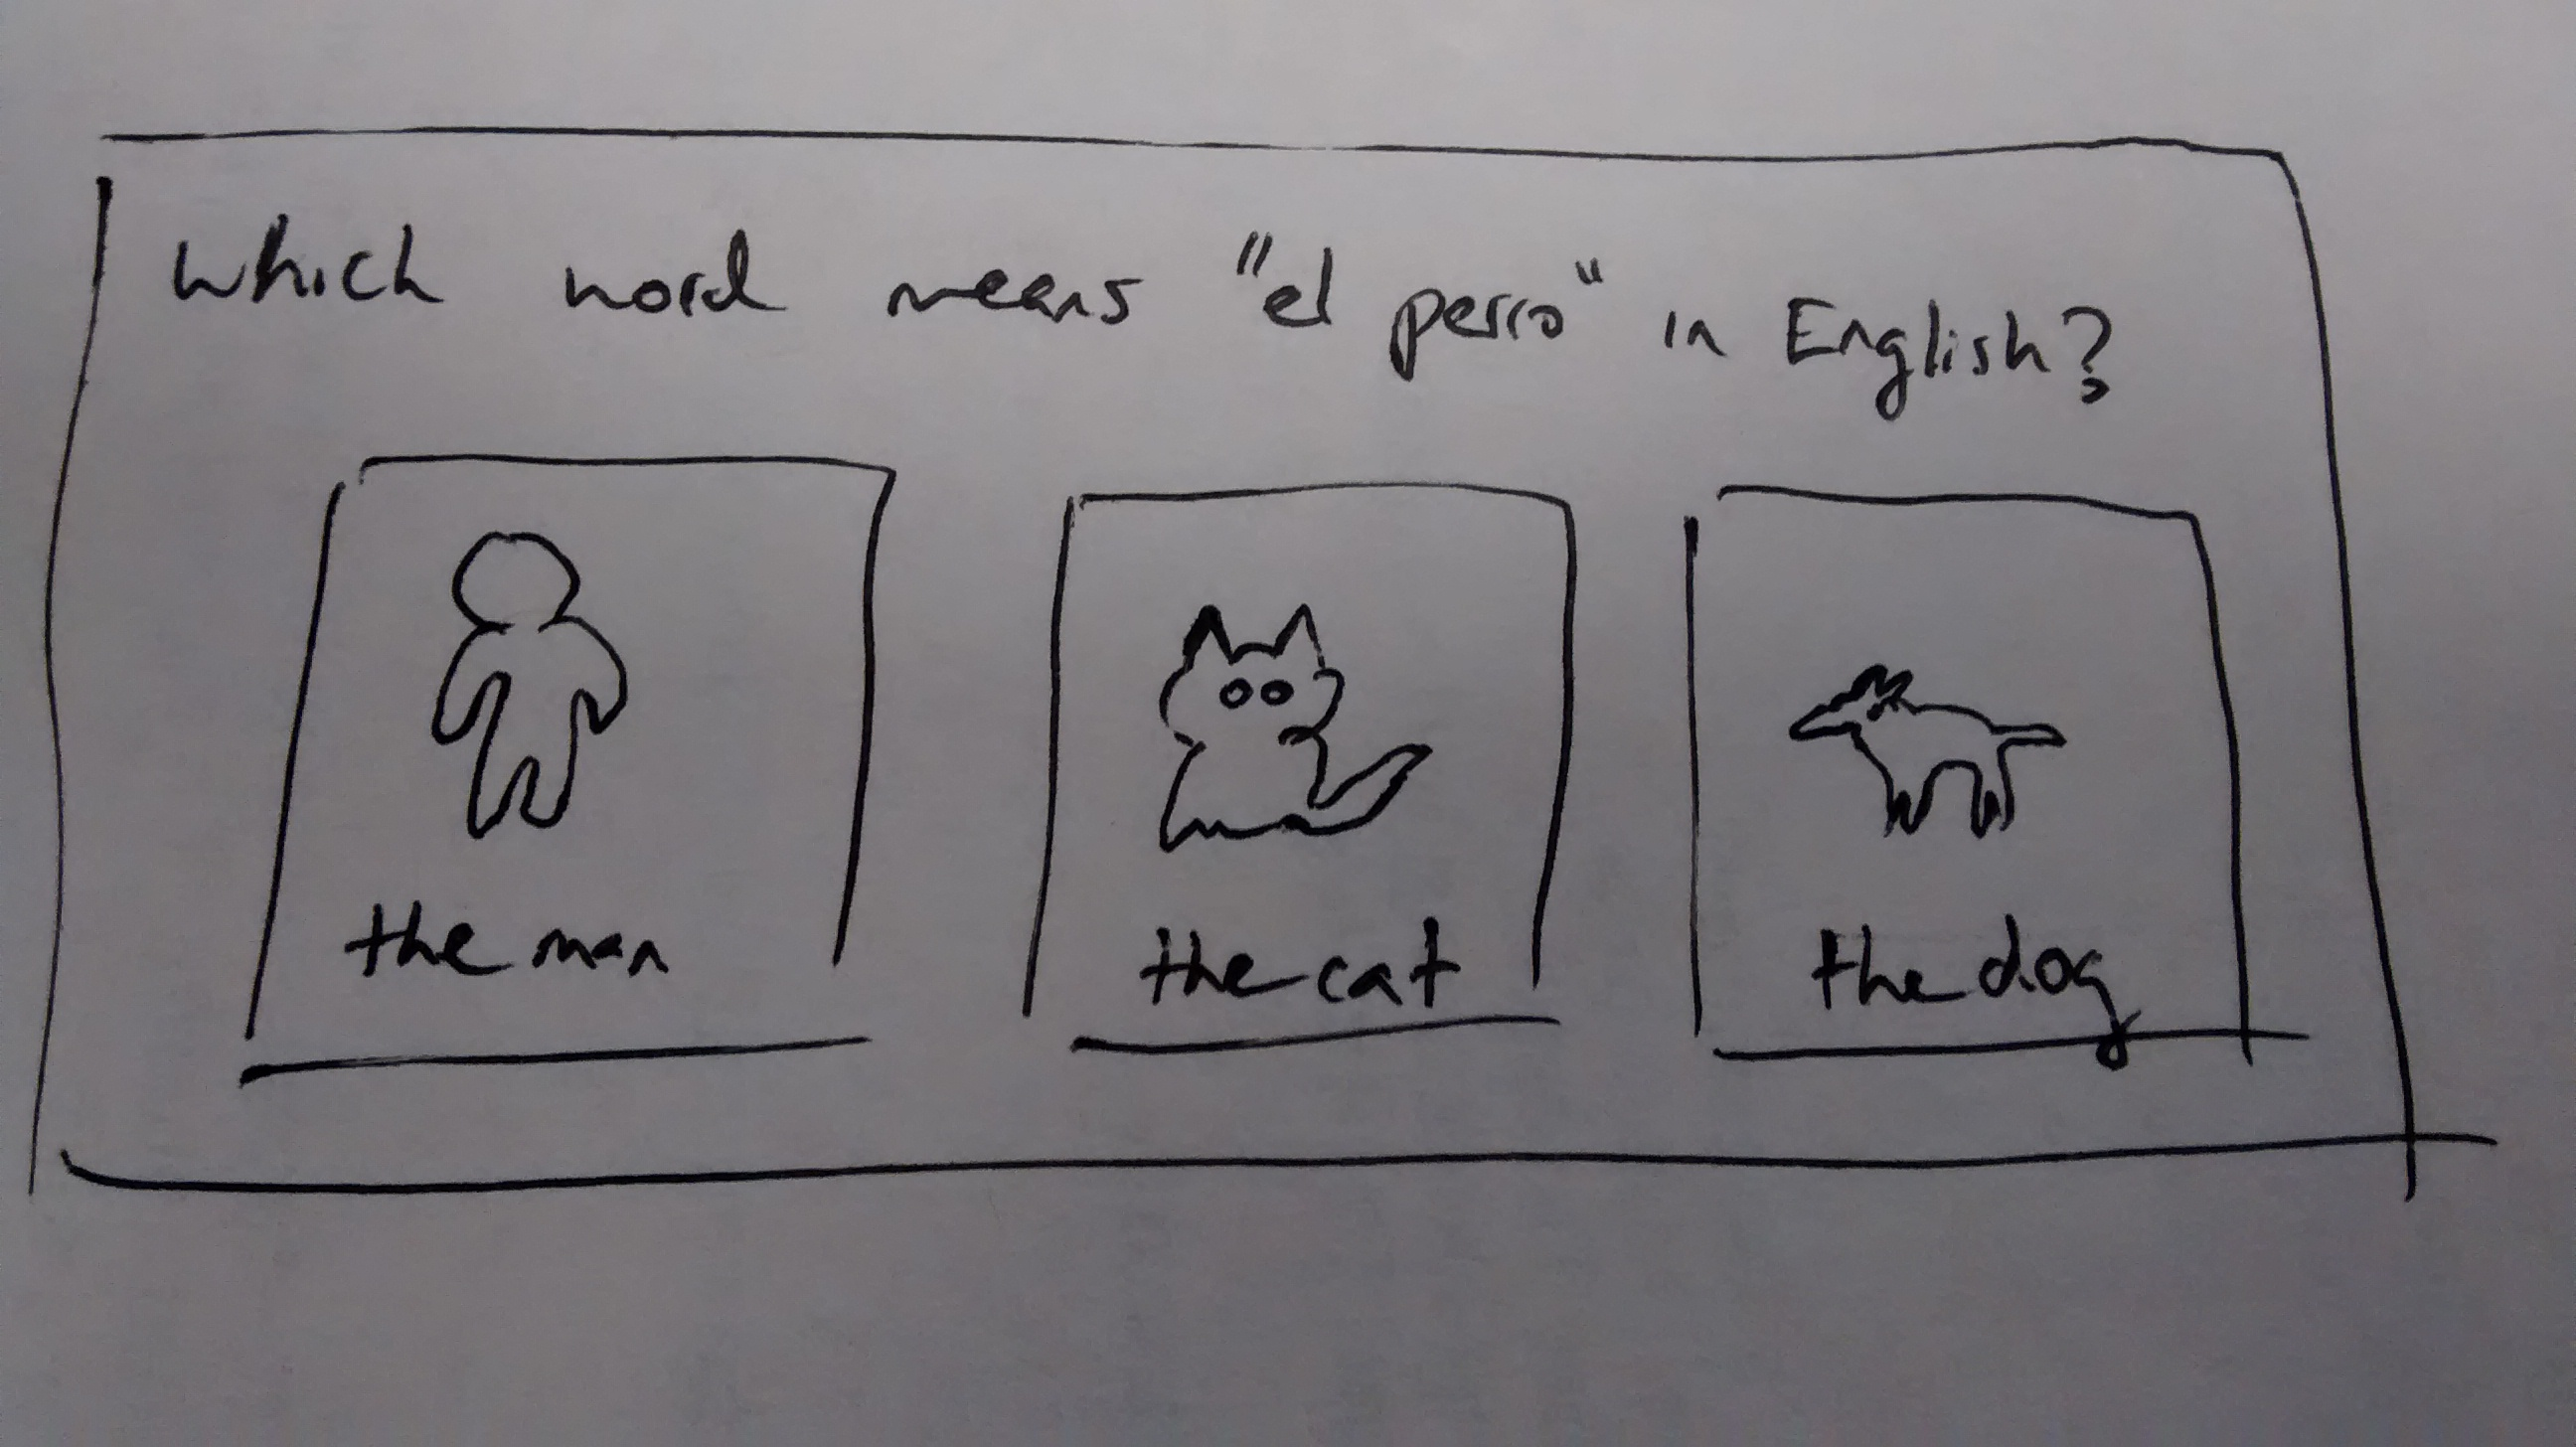
\includegraphics[width=2.0\columnwidth]{quiz2}
\caption{Another type of quiz presents a noun in the foreign language (el perro), and asks the user to select the correct translation into the native language (the dog).}
\label{fig:quiz2}
\end{figure*}

A picture is also presented alongside the foreign-language word, to help learners visually remember them. Prior research has shown that flashcards showing a picture along with the text allow learners to learn vocabulary better than text-only flashcards \cite{multimediavocabulary}. We focus on nouns, because they are the most common type of word -- the majority of words in the Oxford English dictionary are nouns \cite{microlearning} -- and they are relatively easy to visualize. This is the same quiz style used by Duolingo to introduce nouns.

We opt to use this interactive quiz format, rather than simply showing pairs of words and translations or asking users to explicitly recall and type out translations for words, because it allows us to take advantage of the testing effect with a minimal amount of interaction (the user simply needs to click on a picture to answer). If the user answers a quiz correctly, a new quiz testing a different word is shown; in this way, they can engage with the vocabulary for as long a duration as they would like to.

\subsection{Quiz Generation}

Quizzes are generated automatically from the provided English word. The other options are generated by looking up the word in WordNet \cite{wordnet}, to find related words that have similar category and semantics but have different meaning (for example, other animal names). The images are obtained by taking the first result on Google Images. We select the list of words to teach based on their overall usefulness in the language (as judged by word frequency in natural-language text).

\subsection{Spaced Repetition}

We use a spaced-repetition algorithm to ensure that the words are encountered at the appropriate frequency, so that users will remember them.

\subsection{Inserting Quizzes into Feeds}

We insert quizzes into feeds so that they will be encountered at a rate of N quizzes per 100 posts. This is optimal because (need justification).

\section{Evaluation}

We conducted a 2-week between-subjects user study to evaluate the effectiveness of our system in teaching foreign-language vocabulary.

\subsection{Participants}

We recruited 30 college students with no prior exposure to Japanese, who were interested in learning some basic vocabulary in Japanese. All of our participants were regular users of Facebook, spending at least 10 minutes on the site each day.

\subsection{Materials}

We selected the 30 most frequently used non-abstract nouns in Japanese, and generated flashcards automatically for them, according to the procedure described in the Quiz Generation section. We presented vocabulary words in romanized form rather than the standard Japanese orthography, to avoid difficulties resulting from unfamiliarity with the Japanese writing system.

\subsection{Conditions}

There were 3 conditions in our study. We assigned 10 students to each:

\begin{itemize}
\item FeedLearn: We inject the quizzes directly into the user's Facebook news feed
\item External Service with In-Feed Reminders: We inject reminders into the news feed asking users to go visit a website where they can take a quiz. The quiz interface on the external website is identical to the one we would have injected directly into the feeds in the FeedLearn condition. The reminders in the feed occur at the same frequency as the quizzes would have been shown in the feeds. This is intended to resemble the experience that would be seen by users using Duolingo and other educational apps, if the users' friends had also enabled posting into their Facebook feeds.
\item External Service with Daily Email Reminders: We give the user a link to the external quizzing service, and send them a daily email at 10AM asking them to go review vocabulary on the site.
\end{itemize}

\subsection{Procedure}

The study is conducted entirely online. First, we ask the users to take a pre-test, to verify that they do not already know the vocabulary that we intend to teach them. The test is a multiple choice test: there are 30 questions total, with 15 questions where questions where the user is given the foreign-language word and is asked to select the correct English translation, and 15 questions where the user is given a word in English and is asked to select the correct foreign translation.

Then, we have them install our extension have them use the service for 2 weeks (according to the condition they have been assigned to). After the 2 weeks have elapsed, we again ask them to take the vocabulary quiz.

\subsection{Research Questions}

H1: Do users learn more vocabulary in the FeedLearn condition than the other conditions?

H2: Do user engage more (complete more quizzes) in the FeedLearn condition than the other conditions?

H3: Do users enjoy the FeedLearn condition more than the other conditions?

\section{Results}

H1: Hopefully, we find that the amount of vocabulary learned in the FeedLearn condition is greater than the other two conditions

H2: Hopefully, we find the users engage more (complete more quizzes) in the FeedLearn condition than the other conditions.

H3: Hopefully, we find that users find injection of quizzes directly into their Facebook feeds less distracting than injection of reminders for them to visit the site, or email-based reminders.

\section{Discussion}

Although in all 3 conditions, users receive daily reminders to go study vocabulary, we found that users complete more quizzes in the FeedLearn condition, and consequently learn more vocabulary.

Relative to the External Service with In-Feed Reminders condition, we can attribute this to the reduced friction required for the interaction: the user no longer needs to leave their news feed and visit an external service to review vocabulary, so the barrier to engagement is lowered by inserting vocabulary quizzes directly into social feeds.

Relative to the External Service with Email Reminders condition, we can additionally attribute an advantage to being able to catch them when they are idle and free. While the user may be busy at 10AM and not have time when they receive the email to review the vocabulary, and will consequently have to remember to go visit the site at a later time, users in the FeedLearn condition have already indicated that they are free and idle because they are browsing their news feed, and are hence more likely to be available to review vocabulary when they encounter them in their feeds.

Users found the FeedLearn condition more enjoyable and less distracting than the External Service with Email Remdiners condition, because they were able to directly go engage with the quiz content, and were not distracted by unnecessary reminder emails.

\section{Conclusion}

Injecting small, actionable tasks into users' Facebook feeds presents an opportunity to influence behavior. Although we have studied foreign-language vocabulary acquisition in this study, our approaches should be equally applicable to other flashcard-like educational content that takes relatively little effort to consume and could be easily injected and interacted with directly inside a social news feed. One could also use a similar mechanism to encourage other behaviors that need to be done for short periods of time on a daily basis, such as small amounts of exercise.

\bibliographystyle{acm-sigchi}
\bibliography{feedlearn}
\end{document}
